\setlength{\parindent}{10ex}

\documentclass{article}
\usepackage{graphicx}
\usepackage{algorithm2e}

\title{Vulnerability Auditing Through Live Stack Tracing}
\author{Spencer Powell}
\date{\today}

\begin{document}

\maketitle

\section {Overview}

%Make a workflow figure clarify relationship between debugger and monitor which preceeds which?

%TODO: first make the graph; then we will explain it.

The overall workflow of our vulnerability detection toolkit is shown in
%Figure\ref{fig-workflow}
Figure 1.1 and includes four main components: the stack monitor, which monitors and logs stack activiy, the debugger,
which calls functions within a target program, a fuzzer, which supplies constructed random inputs to the program, and a
pattern detector, which uses machine learning to analyze the newly created stack monitor logs and detect vulnerable code
patterns. After the stack monitor invokes the debugger, the debugger will call functions within the program itself, in
an effort to lessen the amount of code executed and increase the path coverage. The debugger is capable of giving
arguments to the given function, which can be randomized by fuzzing. Fuzzing is a method of crafting random inputs for a
program in an effort to explore all paths within a given binary or function. Previously known fuzzing techniques can be
applied to these functions, in an effort to trigger crashes. Exploring all paths through a givent binary is an important
step in this process because a given vulnerability in a binary may not be located within a commonly executed logic path.
The stack monitor maintains a log of stack activity during each execution, which is written to a file. Each time the
fuzzer provides a different input to the program, a new log file is produced and saved. This collection of files is then
sent to the vulnerability detector. The detector uses machine learning to recognize vulnerable patterns in stack
activity, and tags potentially vulnerable sections of machine code.

\begin{figure} \begin{center}
%\vspace{-0.3in}
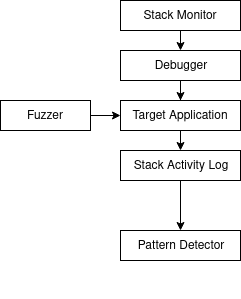
\includegraphics[height=4in]{workflow.png} \end{center}
%\vspace*{-0.3in}
\caption{The Overall Workflow}
%\vspace{-0.4in}
\label{fig-workflow} \end{figure}

\section{The Stack Monitor}

Our stack monitor serves to monitor the execution of an arbitrary program and then creates a log of all the stack
activities, which is later analyzed for vulnerability detection. It takes as input a binary executable of a program
(currently only 64 bit x86 ELF's are supported). The monitor dynamically instruments the user executable to log down the
values of the runtime stack pointer (SP), the base pointer for the stack (BP), and the instruction pointer (IP) before
each instruction is executed. If the instruction reads or writes to memory, instrumentation is inserted to check whether
the targeted memory is within the runtime stack, and if yes, the memory operation is logged. All the logged information
is sent to the stack monitor from the instrumented binary executable using a client-server model for
interprocess-communication.
%An example of the logged information for ??? is illustrated in Figure~\ref{fig-logfile}.
The stack monitor can be configured to either output all the logs into an external file, or in an internal data
structure that can be accessed through python.

% TODO: create figure for stack monitor

\section{The Binary Debugger}

The binary debugger provides an programming interface for the developer to invoke the stack monitor to track any
selected regions of code.  TODO: what is the interface (API)? make a figure and reference the figure. Then try to
explain the logisitics of the API.

\begin{figure} \begin{center}
%\vspace{-0.3in}
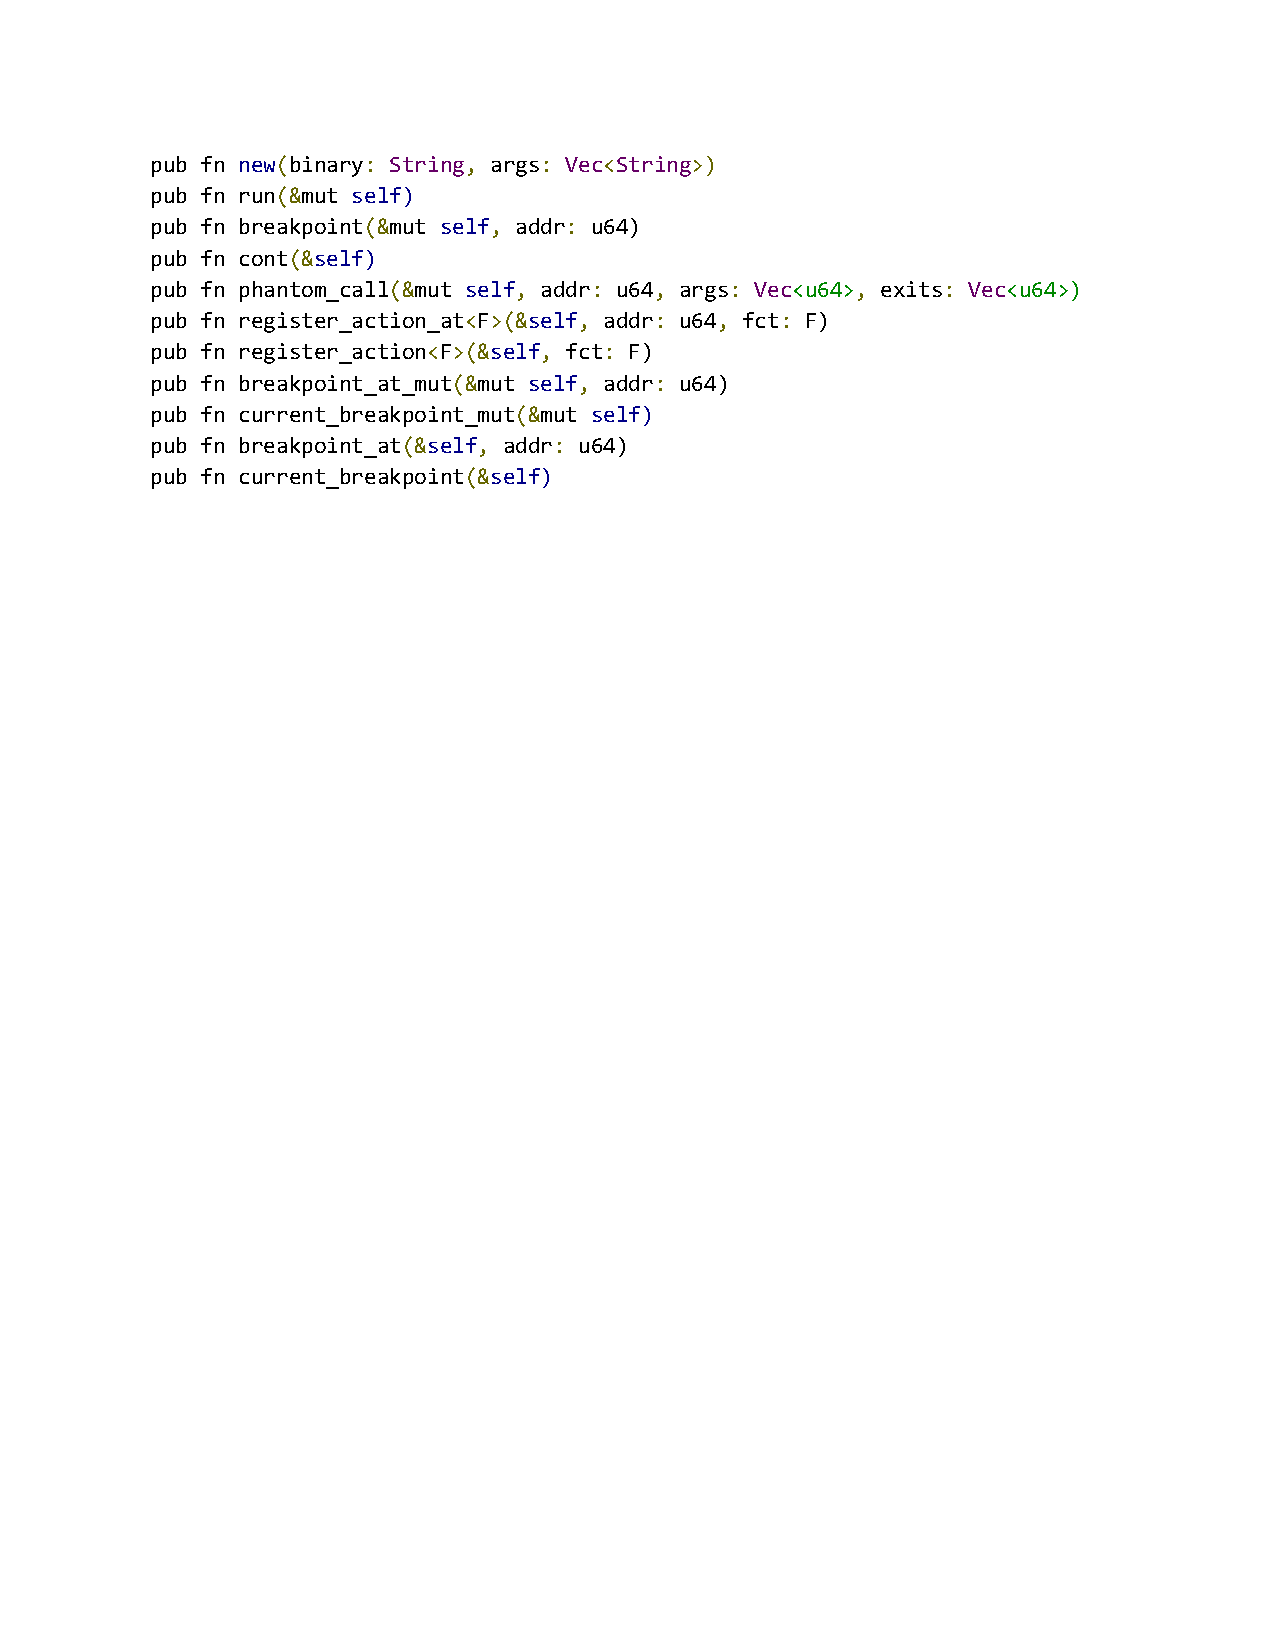
\includegraphics[height=4in]{api.pdf} \end{center}
%\vspace*{-0.3in}
\caption{The Debugger API}
%\vspace{-0.4in}
\label{fig-workflow} \end{figure}

\begin{center}
    \begin{tabular}{|l|l|}
    \hline
    \bf Function & \bf Purpose \\ \hline
    new(path, argv) & Creates a new debugger \\ \hline
    run(self) & Run the debugged program \\ \hline
    breakpoint(self, address) & Add a breakpoint at address \\ \hline
    cont(self) & Continue from current breakpoint \\ \hline
    phantom\_call(self, addr, args, exits) & Construct and call function at addr \\ \hline
    register\_action(self, func) & Register global break action(s) \\ \hline
    register\_action\_at(self, address, func) & Register break action(s) at address \\ \hline
    breakpoint\_at(self, address) & Get reference to breakpoint \\ \hline
    breakpoint\_at\_mut(self, address) & Get mutable reference to breakpoint \\ \hline
    current\_breakpoint(self) & Get reference to current breakpoint \\ \hline
    current\_breakpoint\_mut(self) & Get mutable reference to current breakpoint \\ \hline
    \end{tabular}
\end{center}

The debugger API is compiled into a program, called the debugger, which will spawn a child binary when the run function
is called. The spawned child binary is referred to as the target binary. The API can be used by first creating a
% ugly sentence
Debugger struct with a call to the new() function and providing a path to the target binary with the desired arguments.
The user may then elect to add breakpoints which will be injected into the target binary and cause the target binary to
halt when they are executed. The algorithm used to create the breakpoint can be seen below in figure x.x The
register\_action() and register\_action\_at() functions are provided as a way for the user to execute functions upon
arriving at any breakpoint or a breakpoint which resides at the given address respectively. Upon executing a breakpoint,
the target binary will remain in a dormant state and not execute any more code until the cont() function is called by
the debugger, at which point the target binary will run either until exit or until it arrives at another breakpoint. At
any point when the target binary is dormant at a breakpoint, the user may elect to perform arbitrary function calls in
the target binary by using the phantom\_call() function provided by the debugger. The program will jump to the given
address, initialize the stack frame and program registers according to a predetermined calling convention, and register
cleanup action breakpoints for each address in the exits list. The program will then call the continue() function and
execute the chosen call. Because this function may be called at any point in the code, all registers must be restored to
their original values after the function completes. This action is automatically performed as long as the exit taken by
the desired function is explicitly provided in the exits variable. If the user wishes to modify a breakpoint after it
has been established, they must retrieve it from the debugger with the breakpoint\_at\_mut() function. This will return
a mutable reference to the breakpoint. The sister function breakpoint\_at() function operates similarly, but returns a
read-only reference to the breakpoint.


\begin{algorithm}[H]
    \SetKwInOut{Input}{input}\SetKwInOut{Output}{output}
    \Input{
        Address $A$ in a target binary's text segment \\
    }
    \Output{
        Returns the overwritten data which can be used with the continue algorithm shown in figure x.x \\
    }
    \KwResult{
        A modified text segment which will raise an interrupt if the code at A is executed     \\
    }
    \Begin{
    $data$ := read one WORDSIZE of data from $A$

    $trap$ := $(data \BitAnd \BitNeg \mathrm{0xff})\BitOr\mathrm{0xcc}$;

    write $trap$ to $A$ as a WORDSIZE

    return $data$ \\
    }
    \caption{Adding a breakpoint to a target binary}
\end{algorithm}
\begin{algorithm}[H]
    \SetKwInOut{Input}{input}\SetKwInOut{Output}{output}
    \Input{
        The address $A$ of the current breakpoint \\
        The overwritten instruction $data$ \\
    }
    \Begin{
        write $data$ to $A$ as a WORDSIZE; \\
        set the instruction pointer register = $A$; \\
    }
    \caption{Continuing from a breakpoint in the target binary}
\end{algorithm}

TODO: provide an example of using the API of debugger in the fuzzer. Also the figure will be used to explain the fuzzer.
% do this before ptrace

The programming interface in Figure?? is implemented by making system calls to ptrace. The ptrace system call allows a
process to inspect and manipulate a child process's memory and execution. The arguments for ptrace can be seen in figure
x.x

\begin{center}
    \caption{ptrace(request, pid, addr, data) usage} \\
    \begin{tabular}{|l|l|}
    \hline
    \bf Argument & \bf Purpose \\ \hline
    request & The type of ptrace request, see figure x.x for options \\ \hline
    pid & The process ID of the target binary \\ \hline
    addr & Optional address used for certain values of \bf{request} \\ \hline
    data & Optional data used for certain values of \bf{request} \\ \hline
    \end{tabular}
\end{center}

The debugger spawns a child tracee process by first invoking the fork system call. The child process which results from
the fork call then performs an initial ptrace system call, using the PTRACE\_TRACEME request. This enables the child
process to be traced by a parent tracer process. Breakpoints are set using algorithm shown in % figure xxx

TODO: the specific ptrace call (with interface), TODO: explain how the ptrace interface work. In particular, the
debugger invokes ptrace with the TODO {what requests} to allow the user to monitor and edit the memory of any child
process, to set breakpoints in a child, and to call any function in the child.

%TODO move to potential issues area
The function calls can be constructed with arguments, but no initialization is done to global data. This can be a
potential issue for processes which rely on global variables or preallocated memory. Fake allocations can be performed
by manually allocating space on the stack before calling, but currently the only fix for global variables is to
partially execute sections of the program before executing the desired code.


\section {Path Exploring} Dynamic execution has a few issues with it that must be dealt with. One of the biggest issues
with dynamic execution traces is that of code coverage. Identifying a vulnerability requires that you first execute the
vulnerable piece of code. We have elected to use fuzzing as a technique for code coverage, as it is well researched and
there are many pre-existing methods with which to explore a binary.

\section {The Vunerability Detection} The data from the monitor is analyzed through machine learning, the data must be
preprocessed. The addresses of the stack operations are made to be relative to the base pointer, and the stack frame is
given in an overall size instead of both a stack and base pointer.

\section{Key Technical Challenge}

The key technical challenge of this tool is handling the massive amount of data.  Per instruction, the log contains
three addresses, and extra optional data for memory operations on the stack. This pressents two major issues. The first
issue is the massively increased runtime of the target binary which is required in order to generate the information,
and the second issue is comprehending and manipulating the massive amount of data which is created.

The large influx of data is handled in two distinct methods. The first method is a binary debugger which attempts to
extract and call a given function from a binary. This allows us to limit our scope of analysis to a single area, and
create multiple logs based on differing inputs. The second method used to handle the large dataset is machine learning.
Our goal is to discover patterns in stack behavior could indicate vulnerable logic in a binary. There is far too much
data for this to be done manually, so machine learning was applied.

\end{document}
